\documentclass[border=20pt]{standalone}
\usepackage{tikz}
\usepackage{amsmath}
\usetikzlibrary{calc,arrows.meta}
\begin{document}
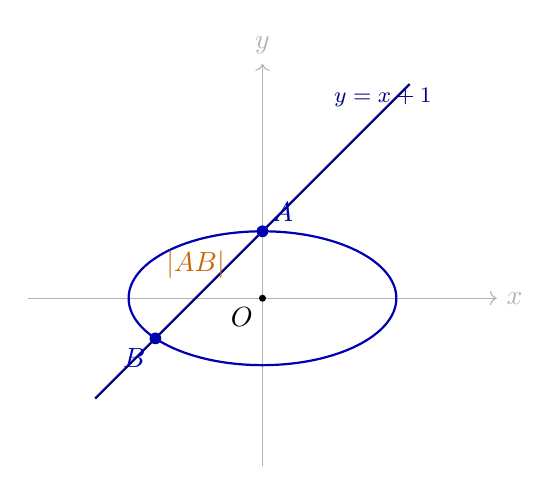
\begin{tikzpicture}[scale=0.85]
  % Axes
  \draw[->, gray!60, thin] (-3.5,0) -- (3.5,0) node[right] {$x$};
  \draw[->, gray!60, thin] (0,-2.5) -- (0,3.5) node[above] {$y$};

  % Ellipse: x^2/4 + y^2 = 1, a=2, b=1
  \draw[thick, blue!70!black] (0,0) ellipse (2 and 1);

  % Line y = x + 1
  % Intersection with ellipse: x^2/4 + (x+1)^2 = 1 → x^2/4 + x^2+2x+1 = 1 → 5x^2/4 + 2x = 0 → x(5x/4+2) = 0
  % x=0 or x=-8/5=-1.6
  % y=1 or y=-0.6
  \coordinate (A) at (0, 1);
  \coordinate (B) at (-1.6, -0.6);

  % The line
  \draw[thick, blue!50!black] (-2.5, -1.5) -- (2.2, 3.2);
  \node[blue!50!black, font=\footnotesize] at (1.8, 3.0) {$y=x+1$};

  % Points
  \fill[blue!70!black] (A) circle (2.5pt) node[above right] {$A$};
  \fill[blue!70!black] (B) circle (2.5pt) node[below left]  {$B$};

  % Origin
  \fill[black] (0,0) circle (1.5pt) node[below left] {$O$};

  % Chord length label
  \node[orange!80!black] at (-1.0, 0.5) {$|AB|$};
\end{tikzpicture}
\end{document}
